% Options for packages loaded elsewhere
% Options for packages loaded elsewhere
\PassOptionsToPackage{unicode}{hyperref}
\PassOptionsToPackage{hyphens}{url}
\PassOptionsToPackage{dvipsnames,svgnames,x11names}{xcolor}
%
\documentclass[
  spanish,
  letterpaper,
  DIV=11,
  numbers=noendperiod]{scrartcl}
\usepackage{xcolor}
\usepackage{amsmath,amssymb}
\setcounter{secnumdepth}{5}
\usepackage{iftex}
\ifPDFTeX
  \usepackage[T1]{fontenc}
  \usepackage[utf8]{inputenc}
  \usepackage{textcomp} % provide euro and other symbols
\else % if luatex or xetex
  \usepackage{unicode-math} % this also loads fontspec
  \defaultfontfeatures{Scale=MatchLowercase}
  \defaultfontfeatures[\rmfamily]{Ligatures=TeX,Scale=1}
\fi
\usepackage{lmodern}
\ifPDFTeX\else
  % xetex/luatex font selection
\fi
% Use upquote if available, for straight quotes in verbatim environments
\IfFileExists{upquote.sty}{\usepackage{upquote}}{}
\IfFileExists{microtype.sty}{% use microtype if available
  \usepackage[]{microtype}
  \UseMicrotypeSet[protrusion]{basicmath} % disable protrusion for tt fonts
}{}
\makeatletter
\@ifundefined{KOMAClassName}{% if non-KOMA class
  \IfFileExists{parskip.sty}{%
    \usepackage{parskip}
  }{% else
    \setlength{\parindent}{0pt}
    \setlength{\parskip}{6pt plus 2pt minus 1pt}}
}{% if KOMA class
  \KOMAoptions{parskip=half}}
\makeatother
% Make \paragraph and \subparagraph free-standing
\makeatletter
\ifx\paragraph\undefined\else
  \let\oldparagraph\paragraph
  \renewcommand{\paragraph}{
    \@ifstar
      \xxxParagraphStar
      \xxxParagraphNoStar
  }
  \newcommand{\xxxParagraphStar}[1]{\oldparagraph*{#1}\mbox{}}
  \newcommand{\xxxParagraphNoStar}[1]{\oldparagraph{#1}\mbox{}}
\fi
\ifx\subparagraph\undefined\else
  \let\oldsubparagraph\subparagraph
  \renewcommand{\subparagraph}{
    \@ifstar
      \xxxSubParagraphStar
      \xxxSubParagraphNoStar
  }
  \newcommand{\xxxSubParagraphStar}[1]{\oldsubparagraph*{#1}\mbox{}}
  \newcommand{\xxxSubParagraphNoStar}[1]{\oldsubparagraph{#1}\mbox{}}
\fi
\makeatother


\usepackage{longtable,booktabs,array}
\newcounter{none} % for unnumbered tables
\usepackage{calc} % for calculating minipage widths
% Correct order of tables after \paragraph or \subparagraph
\usepackage{etoolbox}
\makeatletter
\patchcmd\longtable{\par}{\if@noskipsec\mbox{}\fi\par}{}{}
\makeatother
% Allow footnotes in longtable head/foot
\IfFileExists{footnotehyper.sty}{\usepackage{footnotehyper}}{\usepackage{footnote}}
\makesavenoteenv{longtable}
\usepackage{graphicx}
\makeatletter
\newsavebox\pandoc@box
\newcommand*\pandocbounded[1]{% scales image to fit in text height/width
  \sbox\pandoc@box{#1}%
  \Gscale@div\@tempa{\textheight}{\dimexpr\ht\pandoc@box+\dp\pandoc@box\relax}%
  \Gscale@div\@tempb{\linewidth}{\wd\pandoc@box}%
  \ifdim\@tempb\p@<\@tempa\p@\let\@tempa\@tempb\fi% select the smaller of both
  \ifdim\@tempa\p@<\p@\scalebox{\@tempa}{\usebox\pandoc@box}%
  \else\usebox{\pandoc@box}%
  \fi%
}
% Set default figure placement to htbp
\def\fps@figure{htbp}
\makeatother



\ifLuaTeX
\usepackage[bidi=basic,shorthands=off]{babel}
\else
\usepackage[bidi=default,shorthands=off]{babel}
\fi
\ifLuaTeX
  \usepackage{selnolig} % disable illegal ligatures
\fi


\setlength{\emergencystretch}{3em} % prevent overfull lines

\providecommand{\tightlist}{%
  \setlength{\itemsep}{0pt}\setlength{\parskip}{0pt}}



 


\KOMAoption{captions}{tableheading}
\makeatletter
\@ifpackageloaded{tcolorbox}{}{\usepackage[skins,breakable]{tcolorbox}}
\@ifpackageloaded{fontawesome5}{}{\usepackage{fontawesome5}}
\definecolor{quarto-callout-color}{HTML}{909090}
\definecolor{quarto-callout-note-color}{HTML}{0758E5}
\definecolor{quarto-callout-important-color}{HTML}{CC1914}
\definecolor{quarto-callout-warning-color}{HTML}{EB9113}
\definecolor{quarto-callout-tip-color}{HTML}{00A047}
\definecolor{quarto-callout-caution-color}{HTML}{FC5300}
\definecolor{quarto-callout-color-frame}{HTML}{acacac}
\definecolor{quarto-callout-note-color-frame}{HTML}{4582ec}
\definecolor{quarto-callout-important-color-frame}{HTML}{d9534f}
\definecolor{quarto-callout-warning-color-frame}{HTML}{f0ad4e}
\definecolor{quarto-callout-tip-color-frame}{HTML}{02b875}
\definecolor{quarto-callout-caution-color-frame}{HTML}{fd7e14}
\makeatother
\makeatletter
\@ifpackageloaded{caption}{}{\usepackage{caption}}
\AtBeginDocument{%
\ifdefined\contentsname
  \renewcommand*\contentsname{Tabla de contenidos}
\else
  \newcommand\contentsname{Tabla de contenidos}
\fi
\ifdefined\listfigurename
  \renewcommand*\listfigurename{Listado de Figuras}
\else
  \newcommand\listfigurename{Listado de Figuras}
\fi
\ifdefined\listtablename
  \renewcommand*\listtablename{Listado de Tablas}
\else
  \newcommand\listtablename{Listado de Tablas}
\fi
\ifdefined\figurename
  \renewcommand*\figurename{Figura}
\else
  \newcommand\figurename{Figura}
\fi
\ifdefined\tablename
  \renewcommand*\tablename{Tabla}
\else
  \newcommand\tablename{Tabla}
\fi
}
\@ifpackageloaded{float}{}{\usepackage{float}}
\floatstyle{ruled}
\@ifundefined{c@chapter}{\newfloat{codelisting}{h}{lop}}{\newfloat{codelisting}{h}{lop}[chapter]}
\floatname{codelisting}{Listado}
\newcommand*\listoflistings{\listof{codelisting}{Listado de Listados}}
\makeatother
\makeatletter
\makeatother
\makeatletter
\@ifpackageloaded{caption}{}{\usepackage{caption}}
\@ifpackageloaded{subcaption}{}{\usepackage{subcaption}}
\makeatother
\usepackage{bookmark}
\IfFileExists{xurl.sty}{\usepackage{xurl}}{} % add URL line breaks if available
\urlstyle{same}
% fallback for those not using the hyperref driver hyperxmp:
\makeatletter
\@ifundefined{xmpquote}{\newcommand{\xmpquote}[1]{#1}}{}
\makeatother
\hypersetup{
  pdftitle={El empleo en la Economía del Conocimiento de La Rioja},
  pdfauthor={Lic. en Economía},
  pdflang={es},
  colorlinks=true,
  linkcolor={blue},
  filecolor={Maroon},
  citecolor={Blue},
  urlcolor={Blue},
  pdfcreator={LaTeX via pandoc}}


\title{El empleo en la Economía del Conocimiento de La Rioja}
\usepackage{etoolbox}
\makeatletter
\providecommand{\subtitle}[1]{% add subtitle to \maketitle
  \apptocmd{\@title}{\par {\large #1 \par}}{}{}
}
\makeatother
\subtitle{Diagnóstico 2019-2026}
\author{Lic. en Economía}
\date{septiembre 2026}
\begin{document}
\maketitle

\renewcommand*\contentsname{Tabla de contenidos}
{
\setcounter{tocdepth}{2}
\tableofcontents
}

\section{Resumen ejecutivo}\label{sec-resumen}

El empleo de la Economía del Conocimiento (EC) en La Rioja alcanzó
\textbf{521 puestos en 2025}, equivalente al \textbf{1,93\% del empleo
formal privado provincial}. Sin embargo, de esos 521 puestos, solo
\textbf{63,8 corresponden al núcleo software puro} (consultoría
informática, desarrollo y reparación). El resto (457,6) son
\textbf{proxies}: arquitectura, ingeniería y servicios empresariales.

Cinco hallazgos principales:

\begin{enumerate}
\def\labelenumi{\arabic{enumi}.}
\item
  \textbf{Empleo EC: 521 puestos en 2025 (1,93\% del total provincial).}
  Crecimiento de +46,4\% respecto a 2019, pero con pico en 2023 (513) y
  meseta posterior.
\item
  \textbf{Núcleo software: solo 63,8 puestos (12,2\% del EC).} El 87,8\%
  restante son proxies que no son Economía del Conocimiento en sentido
  estricto.
\item
  \textbf{Prima salarial: +29,0\% sobre el promedio provincial (2025).}
  El núcleo software paga consistentemente por encima del promedio, con
  picos de +53,7\% (2022) y +45,8\% (2024).
\item
  \textbf{El EC resiste mejor la recesión.} En 2025 el empleo EC creció
  +3,0\% mientras el empleo provincial cayó −3,4\%. La participación EC
  subió de 1,32\% (2019) a 1,93\% (2025).
\item
  \textbf{Peor desempeño federal en intensidad.} La Rioja perdió −4,45
  pp de intensidad empresarial EC entre 2022 y 2025, la peor caída de 9
  jurisdicciones comparadas.
\end{enumerate}

\textbf{Diagnóstico general.} El empleo EC de La Rioja tiene un núcleo
de alta calidad (los mejores salarios de la provincia) pero baja escala
(63,8 puestos reales). El desafío no es crear el sector desde cero, sino
escalar las firmas existentes y frenar la pérdida de masa crítica.

\section{Definición y metodología}\label{sec-definicion}

\subsection{Qué es la Economía del
Conocimiento}\label{quuxe9-es-la-economuxeda-del-conocimiento}

La definición utilizada en este informe es la del \textbf{Régimen de
Promoción de la Economía del Conocimiento}, creado por la \textbf{Ley
27.506 (2019)} y modificado por la \textbf{Ley 27.570 (2020)}. Esta ley
identifica las actividades promovidas a partir de códigos de actividad
de la \textbf{Agencia de Recaudación y Control Aduanero (ARCA)} --- ex
AFIP --- y establece beneficios fiscales para las empresas del sector.

\begin{tcolorbox}[enhanced jigsaw, arc=.35mm, bottomrule=.15mm, bottomtitle=1mm, breakable, colback=white, colbacktitle=quarto-callout-note-color!10!white, colframe=quarto-callout-note-color-frame, coltitle=black, left=2mm, leftrule=.75mm, opacityback=0, opacitybacktitle=0.6, rightrule=.15mm, title=\textcolor{quarto-callout-note-color}{\faInfo}\hspace{0.5em}{Nota}, titlerule=0mm, toprule=.15mm, toptitle=1mm]

\textbf{Actualización normativa.} A partir de octubre de 2024, la AFIP
fue disuelta y reemplazada por ARCA (Decreto 953/2024). ARCA es su
continuadora jurídica. La definición del sector EC sigue rigiéndose por
la Ley 27.506, sin cambios.

\end{tcolorbox}

\subsection{Los 8 códigos CIIU
utilizados}\label{los-8-cuxf3digos-ciiu-utilizados}

Para poder cruzar la definición legal con las estadísticas provinciales
disponibles, se tradujeron los códigos ARCA a los códigos \textbf{CIIU
rev. 3} (Clasificador Industrial Internacional Uniforme) que usa el
SIPA-OEDE.

{\def\LTcaptype{none} % do not increment counter
\begin{longtable}[]{@{}
  >{\centering\arraybackslash}p{(\linewidth - 6\tabcolsep) * \real{0.3125}}
  >{\raggedright\arraybackslash}p{(\linewidth - 6\tabcolsep) * \real{0.1875}}
  >{\raggedright\arraybackslash}p{(\linewidth - 6\tabcolsep) * \real{0.1875}}
  >{\centering\arraybackslash}p{(\linewidth - 6\tabcolsep) * \real{0.3125}}@{}}
\toprule\noalign{}
\begin{minipage}[b]{\linewidth}\centering
CIIU
\end{minipage} & \begin{minipage}[b]{\linewidth}\raggedright
Rama
\end{minipage} & \begin{minipage}[b]{\linewidth}\raggedright
Tipo
\end{minipage} & \begin{minipage}[b]{\linewidth}\centering
Datos en La Rioja
\end{minipage} \\
\midrule\noalign{}
\endhead
\bottomrule\noalign{}
\endlastfoot
7210 & Consultores en equipo de informática & Núcleo & s/d \\
7220 & Consultores en informática y suministro de programas & Núcleo SW
& ✅ \\
7250 & Mantenimiento y reparación de maq. oficina/informática & Núcleo
SW & ✅ \\
7290 & Actividades de informática n.c.p. & Núcleo SW & ✅ \\
7300 & Investigación y desarrollo & Núcleo amplio & s/d \\
7421 & Arquitectura e ingeniería & Proxy & ✅ \\
7430 & Servicios de publicidad & Núcleo amplio & s/d \\
7499 & Servicios empresariales n.c.p. & Proxy & ✅ \\
\end{longtable}
}

\textbf{Tipos}: - \textbf{Núcleo software} (7220 + 7250 + 7290):
definición canónica para análisis de empleo calificado. - \textbf{Núcleo
amplio} (+ 7300 + 7430): agrega I+D y publicidad. - \textbf{Proxies}
(7421 + 7499): agrupan actividades que van más allá de la EC estricta.

\begin{tcolorbox}[enhanced jigsaw, arc=.35mm, bottomrule=.15mm, bottomtitle=1mm, breakable, colback=white, colbacktitle=quarto-callout-warning-color!10!white, colframe=quarto-callout-warning-color-frame, coltitle=black, left=2mm, leftrule=.75mm, opacityback=0, opacitybacktitle=0.6, rightrule=.15mm, title=\textcolor{quarto-callout-warning-color}{\faExclamationTriangle}\hspace{0.5em}{Advertencia}, titlerule=0mm, toprule=.15mm, toptitle=1mm]

\textbf{Advertencia metodológica.} Los códigos \textbf{7421}
(arquitectura, ingeniería, geología) y \textbf{7499} (servicios
empresariales: diseño, traducción, cobranzas) son \textbf{proxies}: el
SIPA no permite aislar la actividad EC específica dentro de ellos. Bajo
la definición amplia, el \textbf{87,8\% del empleo EC depende de estos
dos códigos}. El conteo es un \textbf{techo superior}, no un número
exacto.

\end{tcolorbox}

\subsection{Fuente de datos}\label{fuente-de-datos}

{\def\LTcaptype{none} % do not increment counter
\begin{longtable}[]{@{}
  >{\raggedright\arraybackslash}p{(\linewidth - 2\tabcolsep) * \real{0.5000}}
  >{\raggedright\arraybackslash}p{(\linewidth - 2\tabcolsep) * \real{0.5000}}@{}}
\toprule\noalign{}
\begin{minipage}[b]{\linewidth}\raggedright
Concepto
\end{minipage} & \begin{minipage}[b]{\linewidth}\raggedright
Detalle
\end{minipage} \\
\midrule\noalign{}
\endhead
\bottomrule\noalign{}
\endlastfoot
\textbf{Organismo} & SIPA-OEDE (Observatorio de Empleo y Dinámica
Empresarial) \\
\textbf{Dependencia} & Secretaría de Trabajo, Empleo y Seguridad Social
(STEySS) \\
\textbf{Sistema} & Sistema Integrado Previsional Argentino (SIPA) \\
\textbf{Archivo} &
\texttt{provinciales\_serie\_empleo\_trimestral\_4dig\_7.xlsx} \\
\textbf{Hoja} & ``La Rioja'' \\
\textbf{Cobertura} & 1° Trim 1996 -- 4° Trim 2025 \\
\textbf{Unidad} & Puestos de trabajo (stock al cierre del trimestre) \\
\end{longtable}
}

El SIPA es un \textbf{registro administrativo}: todas las empresas
registradas presentan declaraciones juradas mensuales con su personal en
relación de dependencia. No es una encuesta, por lo que tiene cobertura
casi universal del empleo formal.

\section{Cuánto empleo EC hay}\label{sec-cuanto}

\subsection{Serie histórica
2019-2025}\label{serie-histuxf3rica-2019-2025}

\begin{figure}

\centering{

\pandocbounded{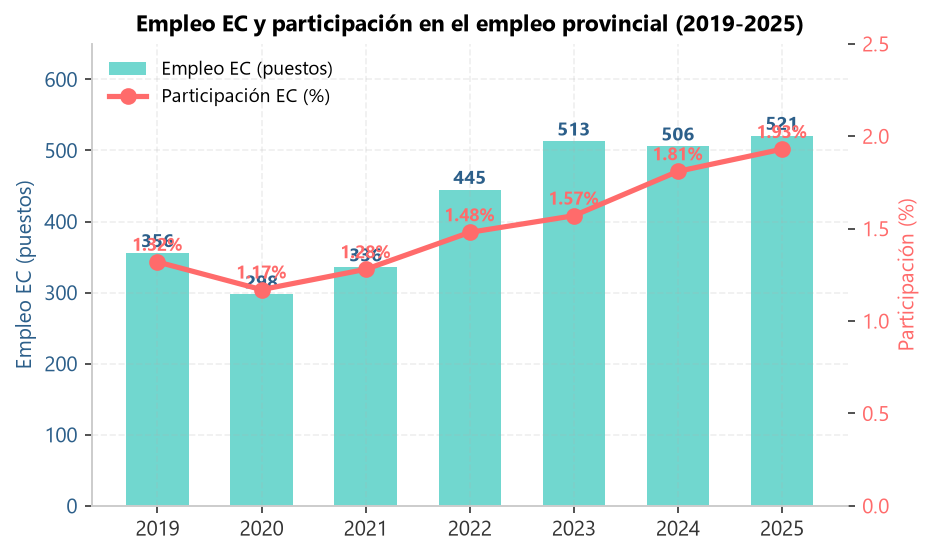
\includegraphics[keepaspectratio]{figuras/F36_empleo_share.png}}

}

\caption{\label{fig-emp-share}Empleo EC y participación en el empleo
provincial (2019-2025).}

\end{figure}%

{\def\LTcaptype{none} % do not increment counter
\begin{longtable}[]{@{}crrr@{}}
\toprule\noalign{}
Año & Empleo EC (8 CIIU) & Empleo provincial total & Participación \\
\midrule\noalign{}
\endhead
\bottomrule\noalign{}
\endlastfoot
2019 & 356 & 26.894 & 1,32\% \\
2020 & 298 & 25.399 & 1,17\% \\
2021 & 336 & 26.245 & 1,28\% \\
2022 & 445 & 30.125 & 1,48\% \\
2023 & 513 & 32.701 & 1,57\% \\
2024 & 506 & 28.008 & 1,81\% \\
2025 & \textbf{521} & \textbf{27.047} & \textbf{1,93\%} \\
\end{longtable}
}

\textbf{Fuente}: SIPA-OEDE (STEySS), CIIU 7210-7499.

El empleo EC pasó de \textbf{356} (2019) a \textbf{521} puestos (2025),
un aumento de \textbf{+46,4\%}. El pico se registró en \textbf{2023} con
513 puestos. Entre 2023 y 2025 el empleo EC creció solo \textbf{+1,6\%},
mientras el empleo provincial caía \textbf{−17,3\%}.

\begin{tcolorbox}[enhanced jigsaw, arc=.35mm, bottomrule=.15mm, bottomtitle=1mm, breakable, colback=white, colbacktitle=quarto-callout-important-color!10!white, colframe=quarto-callout-important-color-frame, coltitle=black, left=2mm, leftrule=.75mm, opacityback=0, opacitybacktitle=0.6, rightrule=.15mm, title=\textcolor{quarto-callout-important-color}{\faExclamation}\hspace{0.5em}{Importante}, titlerule=0mm, toprule=.15mm, toptitle=1mm]

\textbf{Efecto composición.} La participación del EC en el empleo
provincial subió de 1,32\% a 1,93\%. Pero ese aumento se explica, en
parte, por la caída del denominador provincial (−17,3\% entre 2023 y
2025), no solo por crecimiento del sector. En 2024-2025, sin embargo, el
empleo EC creció +3,0\% en términos absolutos, lo que sí es genuino.

\end{tcolorbox}

\subsection{Desglose 2025 por CIIU}\label{desglose-2025-por-ciiu}

{\def\LTcaptype{none} % do not increment counter
\begin{longtable}[]{@{}
  >{\centering\arraybackslash}p{(\linewidth - 14\tabcolsep) * \real{0.1786}}
  >{\raggedright\arraybackslash}p{(\linewidth - 14\tabcolsep) * \real{0.1071}}
  >{\raggedleft\arraybackslash}p{(\linewidth - 14\tabcolsep) * \real{0.1071}}
  >{\raggedleft\arraybackslash}p{(\linewidth - 14\tabcolsep) * \real{0.1071}}
  >{\raggedleft\arraybackslash}p{(\linewidth - 14\tabcolsep) * \real{0.1071}}
  >{\raggedleft\arraybackslash}p{(\linewidth - 14\tabcolsep) * \real{0.1071}}
  >{\raggedleft\arraybackslash}p{(\linewidth - 14\tabcolsep) * \real{0.1071}}
  >{\centering\arraybackslash}p{(\linewidth - 14\tabcolsep) * \real{0.1786}}@{}}
\toprule\noalign{}
\begin{minipage}[b]{\linewidth}\centering
CIIU
\end{minipage} & \begin{minipage}[b]{\linewidth}\raggedright
Rama
\end{minipage} & \begin{minipage}[b]{\linewidth}\raggedleft
T1
\end{minipage} & \begin{minipage}[b]{\linewidth}\raggedleft
T2
\end{minipage} & \begin{minipage}[b]{\linewidth}\raggedleft
T3
\end{minipage} & \begin{minipage}[b]{\linewidth}\raggedleft
T4
\end{minipage} & \begin{minipage}[b]{\linewidth}\raggedleft
\textbf{Promedio 2025}
\end{minipage} & \begin{minipage}[b]{\linewidth}\centering
Tipo
\end{minipage} \\
\midrule\noalign{}
\endhead
\bottomrule\noalign{}
\endlastfoot
7220 & Consultores en informática & 27 & 27 & 28 & 25 & \textbf{26,8} &
Núcleo SW \\
7250 & Mantenimiento y reparación & 6 & 6 & 4 & 1 & \textbf{4,2} &
Núcleo SW \\
7290 & Informática n.c.p. & 29 & 32 & 36 & 34 & \textbf{32,8} & Núcleo
SW \\
7421 & Arquitectura e ingeniería & 172 & 225 & 217 & 197 &
\textbf{202,8} & Proxy \\
7499 & Servicios empresariales & 282 & 235 & 204 & 298 & \textbf{254,8}
& Proxy \\
7210 & Consultores equipo informática & s/d & s/d & s/d & s/d &
\textbf{0} & Núcleo \\
7300 & Investigación y desarrollo & s/d & s/d & s/d & s/d & \textbf{0} &
Núcleo amplio \\
7430 & Servicios de publicidad & s/d & s/d & s/d & s/d & \textbf{0} &
Núcleo amplio \\
& \textbf{TOTAL} & & & & & \textbf{521,4} & \\
\end{longtable}
}

\textbf{Fuente}: SIPA-OEDE (STEySS), hoja ``La Rioja'', promedio simple
de los 4 trimestres de 2025.

\textbf{Los 5 códigos con datos} son 7220, 7250, 7290, 7421 y 7499. Los
otros 3 no registran empleo asalariado privado en La Rioja.

\subsection{Núcleo software
vs.~proxies}\label{nuxfacleo-software-vs.-proxies}

\begin{figure}

\centering{

\pandocbounded{\includegraphics[keepaspectratio]{figuras/empleo_ec_2025_apilado.png}}

}

\caption{\label{fig-desglose}Desglose del empleo EC 2025: núcleo
software vs.~proxies.}

\end{figure}%

{\def\LTcaptype{none} % do not increment counter
\begin{longtable}[]{@{}llrr@{}}
\toprule\noalign{}
Tipo & CIIU & Puestos 2025 & \% del EC \\
\midrule\noalign{}
\endhead
\bottomrule\noalign{}
\endlastfoot
\textbf{Núcleo software} & 7220 + 7250 + 7290 & \textbf{63,8} &
\textbf{12,2\%} \\
\textbf{Núcleo amplio} & 7210 + 7300 + 7430 & 0 & 0,0\% \\
\textbf{Proxies} & 7421 + 7499 & \textbf{457,6} & \textbf{87,8\%} \\
\textbf{TOTAL EC} & & \textbf{521,4} & \textbf{100\%} \\
\end{longtable}
}

\textbf{De cada 8 empleos contabilizados como ``Economía del
Conocimiento'', solo 1 es realmente software puro.}

\subsection{Evolución del núcleo vs.~proxies
(2019-2025)}\label{evoluciuxf3n-del-nuxfacleo-vs.-proxies-2019-2025}

{\def\LTcaptype{none} % do not increment counter
\begin{longtable}[]{@{}crrrr@{}}
\toprule\noalign{}
Año & Núcleo SW & Proxies & Total EC & \% Núcleo \\
\midrule\noalign{}
\endhead
\bottomrule\noalign{}
\endlastfoot
2019 & 11,5 & 344,5 & 356 & 3,2\% \\
2020 & 23,8 & 274,2 & 298 & 8,0\% \\
2021 & 29,0 & 307,0 & 336 & 8,6\% \\
2022 & 65,5 & 379,5 & 445 & 14,7\% \\
2023 & 78,0 & 435,0 & 513 & \textbf{15,2\%} \\
2024 & 61,3 & 444,7 & 506 & 12,1\% \\
2025 & 63,8 & 457,6 & 521 & 12,2\% \\
\end{longtable}
}

El núcleo software \textbf{nunca superó el 15,2\% del total EC}. Entre
2023 y 2025 perdió 3 pp de participación: el sector se ``proxificó''.

\section{Cómo evolucionó el empleo EC}\label{sec-evolucion}

\subsection{Crecimiento 2019-2023}\label{crecimiento-2019-2023}

Entre 2019 y 2023, el empleo EC creció \textbf{+44,1\%} (de 356 a 513
puestos). Ese crecimiento fue impulsado por:

\begin{itemize}
\tightlist
\item
  La recuperación post-pandemia (2021-2022).
\item
  El crecimiento del bloque software, que pasó de 6 a 28 empresas.
\item
  La expansión de consultores informáticos, que multiplicaron por 5 su
  participación en los ingresos del sector.
\end{itemize}

\subsection{La meseta 2024-2025}\label{la-meseta-2024-2025}

Entre 2023 y 2025, el empleo EC pasó de 513 a 521 puestos:
\textbf{+1,6\%}. El sector dejó de crecer.

\textbf{Dos interpretaciones posibles}:

\begin{itemize}
\tightlist
\item
  \textbf{Piso}: el sector tocó fondo y va a recuperarse.
\item
  \textbf{Trampa}: el sector se estabilizó en un nivel bajo sin
  capacidad de recuperación.
\end{itemize}

La evidencia apunta a la segunda: la caída del empleo provincial
(−17,3\% en el mismo período) y la recesión macroeconómica no generan
condiciones para la recuperación.

\subsection{Comparación con el empleo
provincial}\label{comparaciuxf3n-con-el-empleo-provincial}

{\def\LTcaptype{none} % do not increment counter
\begin{longtable}[]{@{}crrr@{}}
\toprule\noalign{}
Período & Empleo EC & Empleo provincial & Diferencia \\
\midrule\noalign{}
\endhead
\bottomrule\noalign{}
\endlastfoot
2023-2025 & \textbf{+1,6\%} & \textbf{−17,3\%} & +18,9 pp \\
\end{longtable}
}

\textbf{El EC resiste mejor la recesión.} En 2025, el empleo EC creció
+3,0\% mientras el empleo provincial cayó −3,4\%. Es un sector con mayor
productividad y menor sensibilidad al ciclo.

\section{Salarios y prima salarial}\label{sec-salarios}

\subsection{Salario por CIIU EC (promedio
2025)}\label{salario-por-ciiu-ec-promedio-2025}

\begin{figure}

\centering{

\pandocbounded{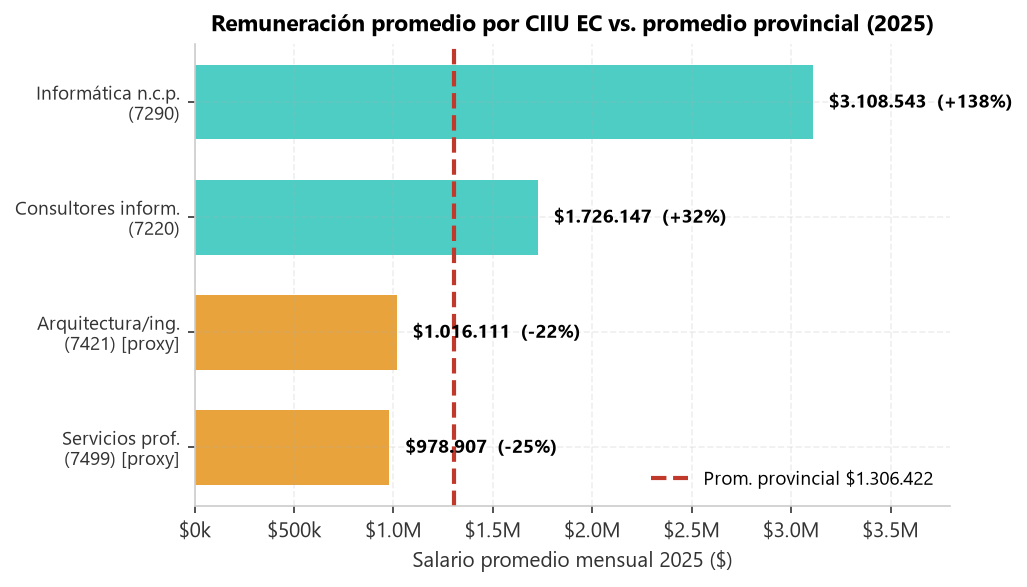
\includegraphics[keepaspectratio]{figuras/F33_salarios_ciiu.png}}

}

\caption{\label{fig-salarios}Remuneración promedio por CIIU EC
vs.~promedio provincial (2025).}

\end{figure}%

{\def\LTcaptype{none} % do not increment counter
\begin{longtable}[]{@{}clrr@{}}
\toprule\noalign{}
CIIU & Rama & Salario promedio 2025 & Prima vs.~provincial \\
\midrule\noalign{}
\endhead
\bottomrule\noalign{}
\endlastfoot
7290 & Informática n.c.p. & \$3.108.543 & \textbf{+138\%} \\
7220 & Consultores informáticos & \$1.726.147 & +32\% \\
7421 & Arquitectura/ingeniería (proxy) & \$1.016.111 & −22\% \\
7499 & Servicios empresariales (proxy) & \$978.907 & −25\% \\
\end{longtable}
}

\textbf{Fuente}: SIPA-OEDE, remuneraciones mensuales por CIIU 4 dígitos,
promedio de los 12 meses de 2025. Salario provincial de referencia:
\$1.306.422.

\textbf{Hallazgo clave}: los dos códigos del núcleo software (7220,
7290) pagan \textbf{por encima} del promedio provincial. Los dos proxies
(7421, 7499) pagan \textbf{por debajo}.

\subsection{Prima salarial del núcleo software
(2022-2025)}\label{prima-salarial-del-nuxfacleo-software-2022-2025}

\begin{figure}

\centering{

\pandocbounded{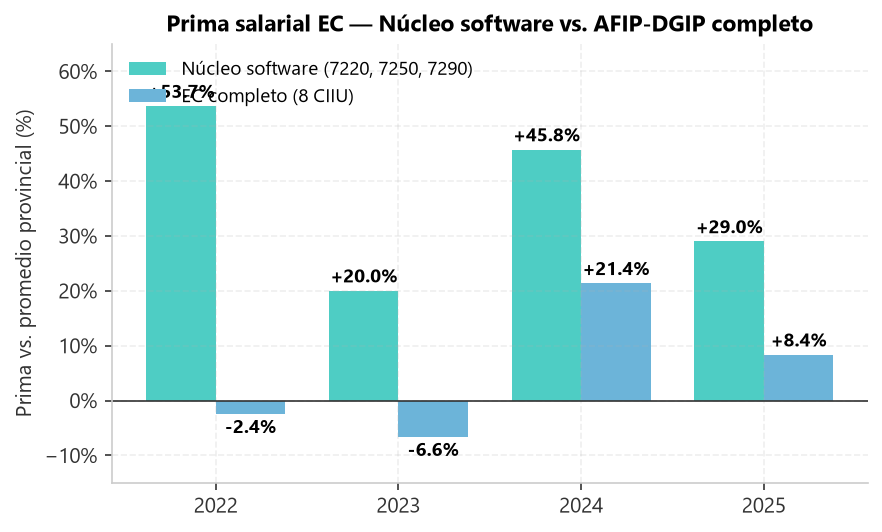
\includegraphics[keepaspectratio]{figuras/F34_prima_salarial.png}}

}

\caption{\label{fig-prima}Prima salarial del núcleo software vs.~EC
completo (2022-2025).}

\end{figure}%

{\def\LTcaptype{none} % do not increment counter
\begin{longtable}[]{@{}crr@{}}
\toprule\noalign{}
Año & Núcleo software & EC completo \\
\midrule\noalign{}
\endhead
\bottomrule\noalign{}
\endlastfoot
2022 & \textbf{+53,67\%} & −2,41\% \\
2023 & \textbf{+20,04\%} & −6,59\% \\
2024 & \textbf{+45,75\%} & +21,38\% \\
2025 & \textbf{+29,00\%} & +8,36\% \\
\end{longtable}
}

La prima del núcleo software se mantuvo \textbf{siempre positiva} en el
período, con un promedio histórico de \textbf{+28,6\%}.

\textbf{Frase clave}: un trabajador del núcleo software gana, en
promedio, \textbf{un 29\% más} que el trabajador promedio de La Rioja.

\section{Comparación federal}\label{sec-federal}

\begin{figure}

\centering{

\pandocbounded{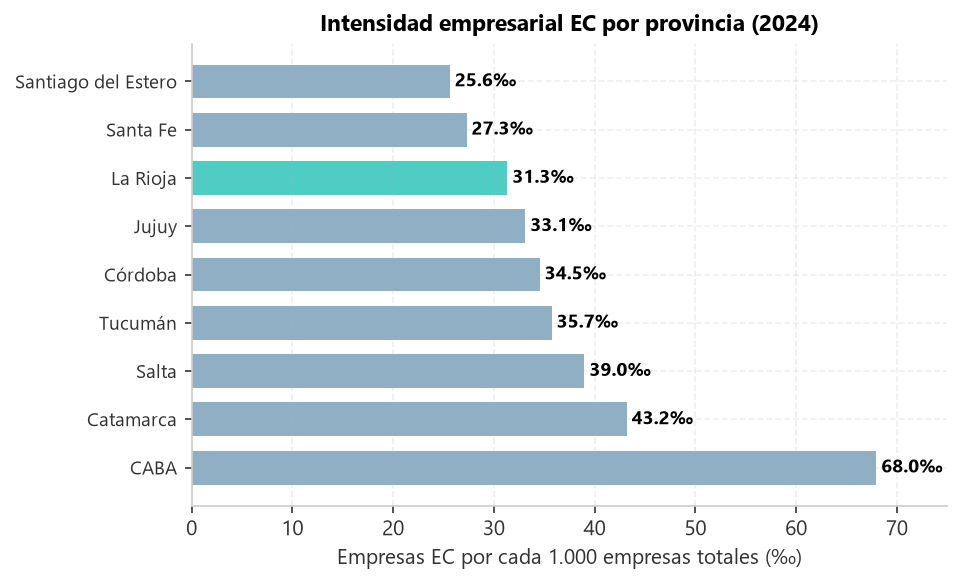
\includegraphics[keepaspectratio]{figuras/F37_intensidad.png}}

}

\caption{\label{fig-intensidad}Intensidad empresarial EC en 9
jurisdicciones (2024). La Rioja en turquesa.}

\end{figure}%

{\def\LTcaptype{none} % do not increment counter
\begin{longtable}[]{@{}lrrrr@{}}
\toprule\noalign{}
Provincia & 2022 & 2024 & 2025 & Δ pp \\
\midrule\noalign{}
\endhead
\bottomrule\noalign{}
\endlastfoot
CABA & 67,30 & 67,95 & 68,64 & +1,34 \\
Catamarca & 39,18 & 43,18 & 44,69 & +5,51 \\
Salta & 37,46 & 38,99 & 42,11 & +4,65 \\
Tucumán & 34,93 & 35,74 & 34,88 & −0,05 \\
Córdoba & 32,81 & 34,55 & 33,90 & +1,09 \\
Jujuy & 31,32 & 33,12 & 32,22 & +0,90 \\
\textbf{La Rioja} & \textbf{33,07} & \textbf{31,34} & \textbf{28,62} &
\textbf{−4,45} \\
Santa Fe & 27,06 & 27,29 & 27,18 & +0,12 \\
Santiago del Estero & 24,31 & 25,63 & 22,24 & −2,07 \\
\end{longtable}
}

\textbf{Intensidad} = empresas EC por cada 1.000 empresas totales.

La Rioja está en el \textbf{7° puesto de 9}. Pero lo más importante es
la \textbf{tendencia}: perdió \textbf{−4,45 pp} entre 2022 y 2025, la
peor caída del grupo.

\textbf{Dato positivo}: La Rioja \textbf{supera a Santa Fe} (27,3‰), una
provincia con una economía 15 veces más grande y con polo tecnológico
consolidado.

\section{Coyuntura y contexto macro}\label{sec-coyuntura}

\begin{figure}

\centering{

\pandocbounded{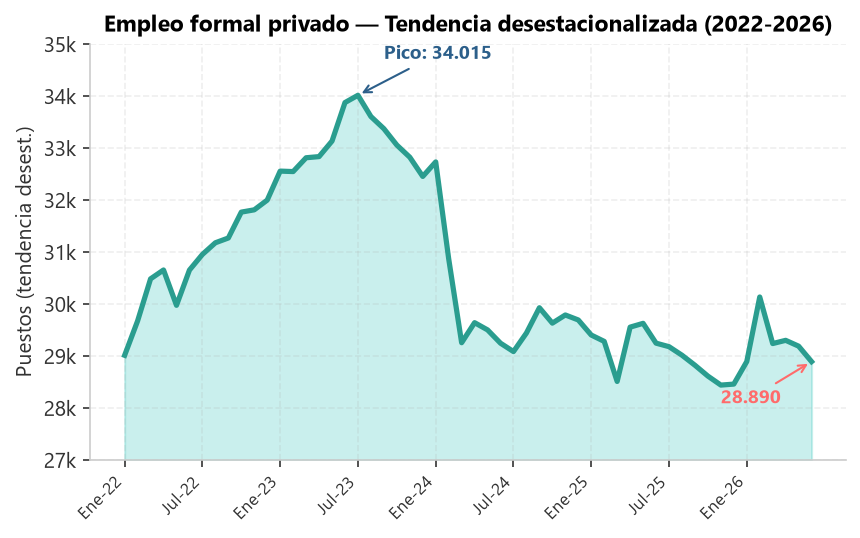
\includegraphics[keepaspectratio]{figuras/F38_empleo_tendencia.png}}

}

\caption{\label{fig-coyuntura}Empleo formal privado --- tendencia
desestacionalizada y variación i.a. (2022-2026).}

\end{figure}%

El empleo privado formal de La Rioja atravesó \textbf{tres fases} entre
2022 y 2026:

\begin{enumerate}
\def\labelenumi{\arabic{enumi}.}
\tightlist
\item
  \textbf{Auge (2022-2023)}: crecimiento post-pandemia, pico en
  \textbf{mayo 2023 (34.329 puestos)}.
\item
  \textbf{Caída (2024)}: derrumbe con variaciones i.a. de hasta
  \textbf{−14,5\%}.
\item
  \textbf{Meseta (2025-2026)}: estabilización en torno a
  \textbf{29.000-30.000 puestos}, con i.a. cerca de cero.
\end{enumerate}

En \textbf{mayo 2026} el stock fue de \textbf{30.305 puestos}, con una
variación interanual de \textbf{−1,7\%}. La caída acumulada desde el
pico histórico (marzo 2017, 38.006) es de \textbf{−24,0\%}.

\textbf{El sector EC resiste mejor que el promedio}: mientras el empleo
provincial cae, el empleo EC crece o se mantiene.

\section{Conclusiones y recomendaciones}\label{sec-conclusiones}

\subsection{Conclusiones}\label{conclusiones}

\begin{enumerate}
\def\labelenumi{\arabic{enumi}.}
\item
  \textbf{Empleo EC: 521 puestos (1,93\% del provincial).} Crecimiento
  de +46,4\% desde 2019, pero con pico en 2023 y meseta posterior.
\item
  \textbf{Núcleo software real: 63,8 puestos (12,2\%).} El resto son
  proxies: arquitectura, ingeniería, servicios empresariales. El conteo
  de 521 es un techo superior.
\item
  \textbf{Prima salarial sostenida: +29,0\% (2025).} El núcleo software
  paga consistentemente por encima del promedio provincial, con promedio
  histórico de +28,6\%.
\item
  \textbf{El EC resiste mejor la recesión.} En 2025, empleo EC +3,0\%
  vs.~empleo provincial −3,4\%.
\item
  \textbf{Peor desempeño federal en tendencia.} La Rioja perdió −4,45 pp
  de intensidad EC entre 2022 y 2025, la peor caída de 9 jurisdicciones.
\end{enumerate}

\subsection{Recomendaciones de
política}\label{recomendaciones-de-poluxedtica}

\begin{enumerate}
\def\labelenumi{\arabic{enumi}.}
\item
  \textbf{Focalizar en el núcleo software} (7220, 7250, 7290). Son 63,8
  puestos reales, no 521. La política pública debería concentrarse en
  esas actividades.
\item
  \textbf{Escalar las 28 empresas de software existentes.} Antes que
  crear nuevas firmas, apuntalar las que ya están. El bloque creció
  +367\% desde 2019 pero cayó a 25 empresas en 2025.
\item
  \textbf{Generar talento local.} La prima del +29\% indica escasez de
  informáticos calificados. Programas de formación específica pueden
  ampliar la oferta y sostener el diferencial.
\item
  \textbf{Aprovechar la ventana de conectividad.} La fibra óptica creció
  +188,7\% en 4 años. Es el soporte físico para captar empleo remoto de
  empresas de otras provincias y del exterior.
\item
  \textbf{Frenar la caída de masa crítica.} El sector perdió −17,6\% de
  empresas entre 2024 y 2025. Sin masa crítica, no hay ecosistema.
\end{enumerate}

\section{Anexo A --- Metodología}\label{sec-anexo}

\subsection{Cómo se calculó el 521}\label{cuxf3mo-se-calculuxf3-el-521}

\textbf{Paso 1} --- Se descargó el archivo
\texttt{provinciales\_serie\_empleo\_trimestral\_4dig\_7.xlsx} del
SIPA-OEDE.

\textbf{Paso 2} --- Se filtró la hoja ``La Rioja''.

\textbf{Paso 3} --- Se seleccionaron los 8 códigos CIIU de la definición
AFIP-DGIP (ahora ARCA-DGIP).

\textbf{Paso 4} --- Para cada código, se tomaron los 4 trimestres de
2025.

\textbf{Paso 5} --- Se calculó el promedio simple de los trimestres con
dato disponible.

\textbf{Paso 6} --- Se sumaron los 8 promedios para obtener el total EC
2025.

\subsection{Limitaciones}\label{limitaciones}

\begin{enumerate}
\def\labelenumi{\arabic{enumi}.}
\item
  \textbf{Proxies 7421 y 7499}: agrupan arquitectura, ingeniería,
  geología, diseño, traducción, cobranzas. No son EC en sentido
  estricto.
\item
  \textbf{Sin datos en 7210, 7300, 7430}: no registran empleo asalariado
  privado en La Rioja.
\item
  \textbf{2025 preliminar}: los datos pueden ser revisados por OEDE.
\item
  \textbf{Salario promedio, no mediana}: sensible a cambios en
  composición.
\item
  \textbf{El 521 es un techo superior}: el núcleo real son 63,8 puestos.
\end{enumerate}

\section{Anexo B --- Siglas y enlaces}\label{sec-siglas}

\subsection{Siglas}\label{siglas}

{\def\LTcaptype{none} % do not increment counter
\begin{longtable}[]{@{}
  >{\raggedright\arraybackslash}p{(\linewidth - 2\tabcolsep) * \real{0.5000}}
  >{\raggedright\arraybackslash}p{(\linewidth - 2\tabcolsep) * \real{0.5000}}@{}}
\toprule\noalign{}
\begin{minipage}[b]{\linewidth}\raggedright
Sigla
\end{minipage} & \begin{minipage}[b]{\linewidth}\raggedright
Significado
\end{minipage} \\
\midrule\noalign{}
\endhead
\bottomrule\noalign{}
\endlastfoot
\textbf{ARCA} & Agencia de Recaudación y Control Aduanero (ex AFIP) \\
\textbf{AFIP} & Administración Federal de Ingresos Públicos (disuelta
2024) \\
\textbf{CIIU} & Clasificador Industrial Internacional Uniforme (rev.
3) \\
\textbf{DGIP} & Dirección General de Ingresos Provinciales (La Rioja) \\
\textbf{EC} & Economía del Conocimiento \\
\textbf{II.BB.} & Ingresos Brutos \\
\textbf{INDEC} & Instituto Nacional de Estadística y Censos \\
\textbf{OEDE} & Observatorio de Empleo y Dinámica Empresarial \\
\textbf{SIPA} & Sistema Integrado Previsional Argentino \\
\textbf{STEySS} & Secretaría de Trabajo, Empleo y Seguridad Social \\
\end{longtable}
}

\subsection{Enlaces a fuentes
oficiales}\label{enlaces-a-fuentes-oficiales}

{\def\LTcaptype{none} % do not increment counter
\begin{longtable}[]{@{}
  >{\raggedright\arraybackslash}p{(\linewidth - 2\tabcolsep) * \real{0.5000}}
  >{\raggedright\arraybackslash}p{(\linewidth - 2\tabcolsep) * \real{0.5000}}@{}}
\toprule\noalign{}
\begin{minipage}[b]{\linewidth}\raggedright
Fuente
\end{minipage} & \begin{minipage}[b]{\linewidth}\raggedright
Enlace
\end{minipage} \\
\midrule\noalign{}
\endhead
\bottomrule\noalign{}
\endlastfoot
SIPA-OEDE (STEySS) &
https://www.argentina.gob.ar/trabajo/estadisticas \\
Ley 27.506 (InfoLEG) &
https://servicios.infoleg.gob.ar/infolegInternet/anexos/320000-324999/324101/texact.htm \\
Ley 27.570 (InfoLEG) &
https://servicios.infoleg.gob.ar/infolegInternet/anexos/340000-344999/341816/norma.htm \\
Decreto 953/2024 (Boletín Oficial) &
https://www.boletinoficial.gov.ar/ \\
ARCA (sitio oficial) & https://www.arca.gob.ar/ \\
DGIP La Rioja & https://www.dgip.larioja.gob.ar/ \\
INDEC & https://www.indec.gob.ar/ \\
\end{longtable}
}

\section{Anexo C --- Serie histórica completa}\label{sec-serie}

{\def\LTcaptype{none} % do not increment counter
\begin{longtable}[]{@{}crrrr@{}}
\toprule\noalign{}
Año & Núcleo SW & Proxies & Total EC & \% Núcleo \\
\midrule\noalign{}
\endhead
\bottomrule\noalign{}
\endlastfoot
2019 & 11,5 & 344,5 & 356 & 3,2\% \\
2020 & 23,8 & 274,2 & 298 & 8,0\% \\
2021 & 29,0 & 307,0 & 336 & 8,6\% \\
2022 & 65,5 & 379,5 & 445 & 14,7\% \\
2023 & 78,0 & 435,0 & 513 & 15,2\% \\
2024 & 61,3 & 444,7 & 506 & 12,1\% \\
2025 & 63,8 & 457,6 & 521 & 12,2\% \\
\end{longtable}
}

\textbf{Fuente}: SIPA-OEDE (STEySS). Elaboración propia.




\end{document}
